\section{Auswertung}
\label{sec:Auswertung}

\subsection{Verifizierung der Linsengleichung}
Die gemessenen Bild- und Gegenstandslängen sind in Tabelle (\ref{tab:einzel1}) zu finden. Aus diesen Größen wird jeweils mit Gleichung (\ref{eqn:linsengleichung})
die Brennweite $f$ für  die Linse berechnet. Auch diese sind in selbiger Tabelle aufgelistet.
Verwendet wurde eine Linse, welche laut Herstellerangabe eine Brennweite von $f = 100\si{\milli\meter}$ besitzt.
\begin{table}[H]
\centering
\caption{Bild-und Gegenstandsweite und zugehörige Brennweite.}
\label{tab:einzel1}
\begin{tabular}{c c c}
\toprule
$g/\si{\milli\meter}$ & $b/\si{\milli\meter}$ & $f/\si{\milli\meter}$\\
\midrule
280  &	151 & 98,10 \\ 
260  &	158 & 98,28 \\
240  &	166 & 98,13 \\
220  &	175 & 97,47 \\
200  &	193 & 98,22 \\
180  &	217 & 98,39 \\
160  &	250 & 97,56 \\
140  &	317 & 97,11 \\
300  &	146 & 98,21 \\
320  &	144 & 99,31 \\
\bottomrule
\end{tabular}
\end{table}

Der Mittelwert und zugehöriger Fehler der Brennweiten berechnet sich durch
\begin{align*}
x &= \frac{1}{10}\cdot \sum_{n=1}^{10} x_i\\
\Delta x &=\frac{1}{\sqrt{10}} \cdot \sqrt{\frac{1}{9} \sum_{n=1}^{10} (x_i - x)^2} 
\end{align*}
Somit lautet die Brennweite der Linse
\begin{align*}
f_1 = (98,08 \pm 0,57) \si{\milli\meter} .
\end{align*}

Um graphisch die Brennweite zu bestimmen, werden die $b$- und $g$-Wertepaare aus Tabelle (\ref{tab:einzel1}) in ein Diagramm eingezeichnet und durch eine Gerade verbunden.
Dies ist in Abbildung \ref{fig:plot1} dargestellt.

\begin{figure}[H]
  \centering
  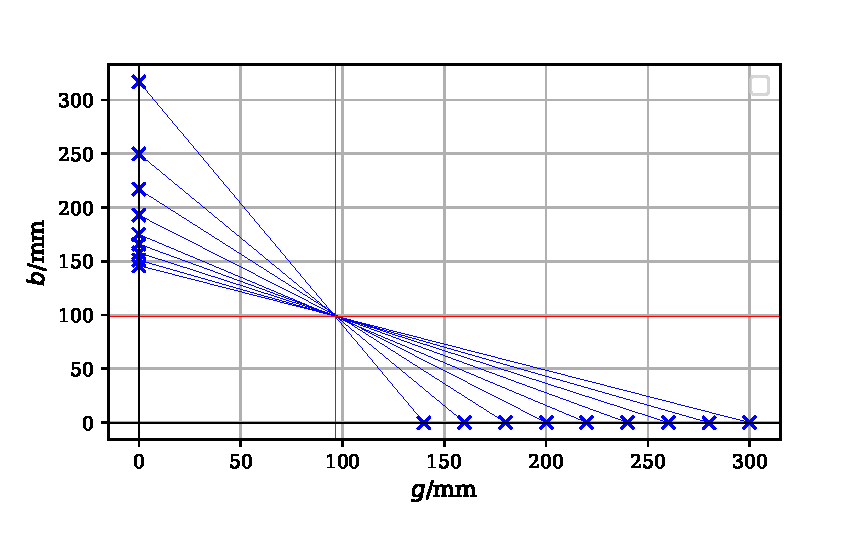
\includegraphics{plot1.pdf}
  \caption{Darstellung der Geraden zwischen Gegenstandsweite und zugehöriger Bildweite.}
  \label{fig:plot1}
\end{figure}

Aus dem Schnittpunkt aller Geraden kann die Brennweite abgelesen werden. Legt man eine horizontale und eine vertikale Linie durch den Schnittpunkt, symbolisiert der jeweilie Achsenschnittpunkt die Brennweite. Im Idealfall ist der Wert auf beiden Achsen identisch.
Da die Schnittpunkte mit den Achsen nicht den gleichen Wert ergeben, ergeben sich ungefähre Werte von $f_x = 96,5 \si{\milli\meter}$ und $f_y = 99\si{\milli\meter}$. Der gemittelte  Wert beträgt $f = (97,75 \pm 1,25)\si{\milli\meter}$.


\subsection{Bestimmung der Brennweite einer Linse durch Bessel}
Für diese Methode wird aus dem Abstand $e$ des Gegenstands und des Bildes und aus der Größe $d_1 = g_1-b_1$ beziehungsweise $d_2 = g_2-b_2$ die Brennweite bestimmt.
Die Messwerte für beide Gegenstands-und Bildweiten sind in Tabelle (\ref{tab:einzel2}) aufgelistet.
\begin{table}[H]
\centering
\caption{Daten zur Bestimmung der Brennweite für weißes Licht.}
\label{tab:einzel2}
\begin{tabular}{c c c c c}
\toprule
$e/\si{\milli\meter}$ & $b1/\si{\milli\meter}$ & $g1/\si{\milli\meter}$ & $b2/\si{\milli\meter}$ & $g2/\si{\milli\meter}$ \\
\midrule
500 &135	& 365	& 369	& 131\\
520 &133	& 387	& 392	& 128\\
540 &131	& 409	& 414	& 126\\
560 &126	& 434	& 437	& 123\\
580 &127	& 453	& 457	& 123\\
600 &124	& 476	& 480	& 120\\
620 &122	& 498	& 500	& 120\\
640 &123	& 517	& 522	& 118\\
660 &121	& 539	& 542	& 118\\	
680 &120	& 560	& 563	& 117\\
\bottomrule
\end{tabular}
\end{table}

Die berechnete Größe $d$ und die zugehörige Brennweite bestimmt durch Gleichung (\ref{eq:bessel}) sind in Tabelle (\ref{tab:einzel3}) zu finden.
\begin{table}[H]
\centering
\caption{Abstand $d_W$ der Linsen und berechnete Brennweiten $f_W$.}
\label{tab:einzel3}
\begin{tabular}{c c c c}
\toprule
$d_{W1}/\si{\milli\meter}$ & $f_{W1}/\si{\milli\meter}$ & $d_{W2}/\si{\milli\meter}$ & $f_{W2}/\si{\milli\meter}$ \\
\midrule
-230 & 98,55 & 238 & 96,68\\
-254 & 98,98 & 264 & 96,49\\
-278 & 99,22 & 288 & 96,60\\
-308 & 97,65 & 314 & 95,98\\
-326 & 99,19 & 334 & 96,92\\
-352 & 98,37 & 360 & 96,00\\
-376 & 97,99 & 380 & 96,77\\
-394 & 99,36 & 404 & 96,24\\
-418 & 98,82 & 424 & 96,90\\
-440 & 98,82 & 446 & 96,87\\
\bottomrule
\end{tabular}
\end{table}

Die Mittelwerte der Brennweiten ergeben sich zu
\begin{align*}
f_{W1} = (98,70 \pm 0,53) \si{\milli\meter}, \\
f_{W2} = (96,55 \pm 0,34) \si{\milli\meter} .
\end{align*}


Gleiches Verfahren wird nun für rotes Licht angewendet. Die Daten befinden sich in Tabelle \ref{tab:einzel4} und die berechneten Größen in Tabelle \ref{tab:einzel5}.


\begin{table}[H]
\centering
\caption{Daten zur Bestimmung der Brennweite für rotes Licht.}
\label{tab:einzel4}
\begin{tabular}{c c c c c}
\toprule
$e/\si{\milli\meter}$ &$b1/\si{\milli\meter}$ & $g1/\si{\milli\meter}$ & $b2/\si{\milli\meter}$ & $g2/\si{\milli\meter}$ \\
\midrule
500 &138 & 362 & 368 & 132\\
550 &130 & 420 & 423 & 127\\
600 &128 & 472 & 478 & 122\\
650 &124 & 526 & 532 & 118\\
700 &122 & 578 & 584 & 116\\
\bottomrule
\end{tabular}
\end{table}

\begin{table}[H]
\centering
\caption{Abstand $d_R$ der Linsen und berechnete Brennweiten $f_R$ für rotes Licht.}
\label{tab:einzel5}
\begin{tabular}{c c c c}
\toprule
$d_{R1}/\si{\milli\meter}$ & $f_{R1}/\si{\milli\meter}$ & $d_{R2}/\si{\milli\meter}$ & $f_{R2}/\si{\milli\meter}$ \\
\midrule
224 & 99,91 & -236 & 97,15\\
290 & 99,27 & -296 & 97,67\\
344 & 100,69 & -356 & 97,19\\
402 & 100,34 & -414 & 96,58\\
456 & 100,74 & -468 & 96,78\\
\bottomrule
\end{tabular}
\end{table}

Die Mittelwerte der Brennweiten für rotes Licht ergeben sich zu
\begin{align*}
f_{R1} = (100,19 \pm 0,55) \si{\milli\meter}, \\
f_{R2} = (97,08 \pm 0,38) \si{\milli\meter} .
\end{align*}

 \noindent Die Daten und die berechneten Größen für blaues Licht befinden sich in Tabellen (\ref{tab:einzel6}) und (\ref{tab:einzel7}). Wieder wird analog verfahren.


\begin{table}[H]
\centering
\caption{Daten zur Bestimmung der Brennweite für blaues Licht.}
\label{tab:einzel6}
\begin{tabular}{c c c c c}
\toprule
$e/\si{\milli\meter}$ &$b1/\si{\milli\meter}$ & $g1/\si{\milli\meter}$ & $b2/\si{\milli\meter}$ & $g2/\si{\milli\meter}$ \\
\midrule
500 &134 & 366 & 369 & 131\\
550 &130 & 420 & 425 & 125\\
600 &124 & 476 & 480 & 120\\
650 &121 & 529 & 533 & 117\\
700 &117 & 583 & 585 & 115\\
\bottomrule
\end{tabular}
\end{table}

\begin{table}[H]
\centering
\caption{Abstand $d_B$ der Linsen und berechnete Brennweiten $f_B$ für blaues Licht.}
\label{tab:einzel7}
\begin{tabular}{c c c c}
\toprule
$d_{B1}/\si{\milli\meter}$ & $f_{B1}/\si{\milli\meter}$ & $d_{B2}/\si{\milli\meter}$ & $f_{B2}/\si{\milli\meter}$ \\
\midrule
232 & 98,09 & -238 & 96,68\\
290 & 99,27 & -300 & 96,59\\
352 & 98,37 & -360 & 96,00\\
408 & 98,48 & -416 & 95,94\\
466 & 97,44 & -470 & 96,11\\
\bottomrule
\end{tabular}
\end{table}

Die Mittelwerte der Brennweiten für blaues Licht ergeben sich zu
\begin{align*}
f_{B1} = (98,33 \pm 0,59) \si{\milli\meter}, \\
f_{B2} = (96,26 \pm 0,31) \si{\milli\meter} .
\end{align*}

\subsection{Bestimmung der Brennweite eines Linsensystems durch Abbe}
Das Linsensystem besteht aus einer Sammellinse mit Brennweite $f_S = 100 \si{\milli\meter}$ und einer Zerstreuungsline mit Brennweite $f_Z = - 100 \si{\milli\meter}$.
Die gemessenen Gegenstands-und Bildweiten und die Bildgröße sind in Tabelle (\ref{tab:einzel8}) aufgelistet. Die Gegenstandsgröße beträgt $G = 28 \si{\milli\meter}$.

\begin{table}[H]
\centering
\caption{Gemessene Bild-und Gegenstandsweite und zugehörige Bildgröße.}
\label{tab:einzel8}
\begin{tabular}{c c c}
\toprule
$g'/\si{\milli\meter}$ & $b'/\si{\milli\meter}$ & $B/\si{\milli\meter}$\\
\midrule
300&	458&	24\\
280&	488&	28\\
290&	478&	26\\
270&	498&	30\\
260&	509&	31\\
250&	515&	33\\
240&	534&	35\\
230&	557&	38\\
220&	575&	42\\
210&	593&	45\\
\bottomrule
\end{tabular}
\end{table}

In einem Diagramm wird $g'$ gegen $1+1/V$ aus Gleichung (\ref{eq:abbe1}) aufgetragen und eine lineare Ausgleichsrechnung durchgeführt(s. Abbildung (\ref{fig:plot2})). Die Größe $V$ berechnet sich mit Hilfe von Gleichung (\ref{eqn:abbildungsgesetz}).
Aus den Parametern der Ausgleichsgeraden lassen sich dann Brennweite und Hauptebenen ablesen.
\begin{figure}[H]
  \centering
  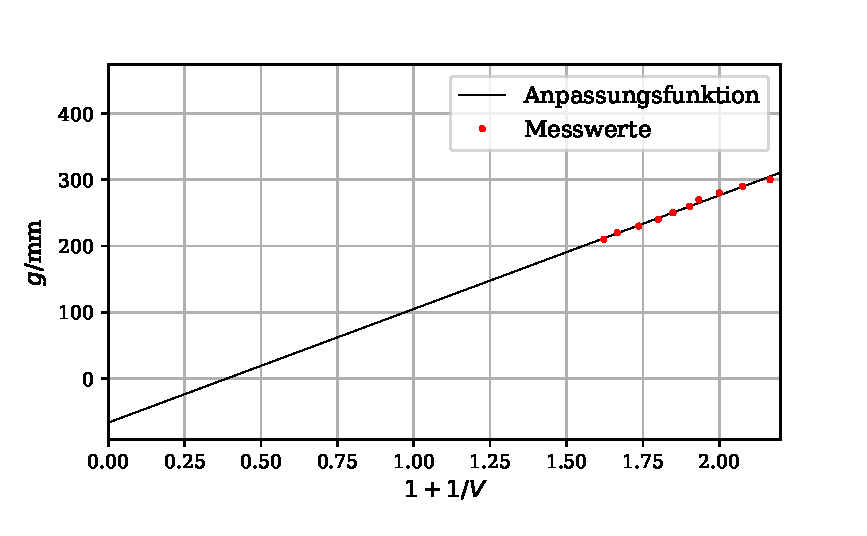
\includegraphics{plot2.pdf}
  \caption{Gegenstandsweite aufgetragen gegen $1+1/V$ und lineare Ausgleichsgerade.}
  \label{fig:plot2}
\end{figure}
Die Parameter der Ausgleichsrechnung betragen
\begin{align*}
a &= f = (171,39 \pm 5,71)\si{\milli\meter},\\
b &= h = (-66,42\pm 10,75)\si{\milli\meter}
\end{align*}


\noindent Außerdem wird $b'$ gegen $1+V$ aus Gleichung (\ref{eq:abbe2}) aufgetragen und erneut eine lineare Ausgleichsrechnung durchgeführt(s. Abbildung (\ref{fig:plot3})).
\begin{figure}[H]
  \centering
  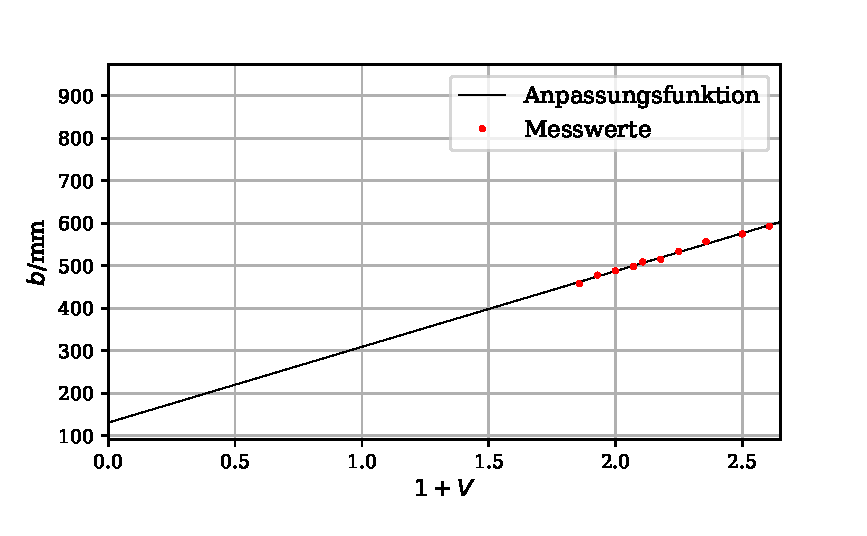
\includegraphics{plot3.pdf}
  \caption{Bildweite aufgetragen gegen $1+V$ und lineare Ausgleichsgerade.}
  \label{fig:plot3}
\end{figure}
Die Parameter der Ausgleichsrechnung betragen
\begin{align*}
a &= f = (178,19 \pm 4,92)\si{\milli\meter},\\
b &= h'= (131,03\pm 10,82)\si{\milli\meter}.
\end{align*}

\noindent Da das System aus einer Sammel- und einer Zerstreuungslinse besteht, kann sich über Matrizenoptik die theoretische Brennweite $f_T$ berechnen über
\begin{align*}
f_T = -\frac{f_{\symup{S}}\cdot f_{\symup{Z}}}{d}.
\end{align*}
Die Größe $d = 60 \si{\milli\meter}$ ist der Abstand der beiden Linsen.
Dies ergibt einen Theoriewert von 
\begin{align*}
f_T = 166,67 \si{\milli\meter}.
\end{align*}
